\subsection{Design method} \label{design_method}
The method used in this study is the Ampersand method.
The Ampersand method is based on relational algebra.
Ampersand makes it possible to make a conceptual analysis of problems. The data model created thereby makes it possible to accelerate implementation.


\subsubsection{Relation Algebra} \label{relation_algebra}
The field of the relation algebra, founded by De Morgan, focuses on operations with sets.
The signature item of relational algebra is the relationship, as the name implies.
This relationship has several properties, namely the attributes.
The attributes in the example of \acrshort{big} would be the surname, first names, gender, date of birth, nationality and address of the person concerned and the number and time of registration~\footnote{\acrlong{big} article 3, paragraph 2}.
In addition, the relationship consists of tuples.
Since the relationship is always between two objects, this is called 2-tuples.
The tuples contain the attributes of the relation.

Basically the operations on sets are the following:
\begin{itemize}
    \item Union, $R \cup S$ %vereniging
    \item Intersection, $R \cap S$ %doorsnede
    \item Difference, $R - S$ or $S - R$ %verschil
\end{itemize}
A distinction must be made between relation algebra and relational algebra.
Ampersand uses relation algebra, so is tuple related and the relational algebra is the foundation of e.g. relational databases.
This includes projections, selections and joins.
The latter are therefore not part of relation algebra.


\subsubsection{Ampersand} \label{ampersand}
Ampersand is based on relation algebra and focuses on business rules~\citepNonPub{wedemeijer_l_joosten_smm_michels_garkenbout_jlc_werkboek_ontwerpen_met_bedrijfsregelspdf_nodate}.
Ampersand supplies correct information systems.
In this case, Ampersand's goal is to provide a correct registry system.
Ampersand's other strengths are its support for conceptual analysis.
It is a platform for reactive programming and generates prototypes.
Ampersand describes the goals rather than the steps.

Business rules are there to pursue a common goal.
These rules are converted into an information system. 
The Ampersand method ensures that when a precise set of rules has been established, an information system can be generated. 
Ampersand focuses on business rules.
To learn how Ampersand works in real life, we design a registry in Ampersand that implements the \acrshort{big}~\citepNonPub{van_wet_2018} .

\begin{wrapfigure} {r}{0.52\textwidth} 
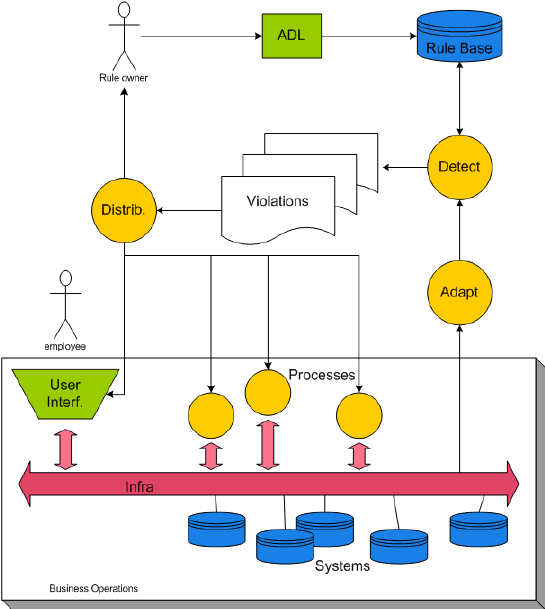
\includegraphics[width=7cm, height=6cm]{04_images/Principle-of-rule-based-process-management.png}
\caption{rule-based-proces}
\label{fig:rule-based-proces}
\end{wrapfigure}


The principle of rule-based \acrfull{bpm} as mentioned in \citepNonPub{joosten_joosten} is that any violation of a business rule may be used to trigger actions. 
This is described in the section \nameref{reactive_approach}.

Ampersand consists of concepts that in turn consist of atoms.
An atom is an implementation of the concept.
Inside the \acrshort{big} is a concept "beroep" with associated atoms like "arts, tandarts, etc".
The concepts are given a name, and the name must be recognized by the business.
This also applies to the definition and purpose of the concepts.
These attributes are not mandatory, but when one wants to generate a functional design, these descriptions of the attributes are very useful.
\begin{lstlisting}[language=Octave] 
CONCEPT Beroep "Beroep van een persoon zoals bedoeld in de wet" 
PURPOSE CONCEPT Beroep 
{+Beroep dat uitgeoefend wordt+}
POPULATION Beroep CONTAINS [
    "arts",
    "tandarts",
    "apotheker",
    "gezondheidszorgpsycholoog",
    "psychotherapeut",
    "fysiotherapeut",
    "verloskundige",
    "verpleegkundige",
    "physician assistant",
    "orthopedagoog-generalist"
]
\end{lstlisting}

Concepts can have relationships with each other.
If the data of the concepts is true and the rules yield consistent data then the relationships between real data are facts.
These facts together form one truth.
Not all concepts are directly related.
Within the domain of the \acrshort{big} we could distinguish the concept of "registratie" and the concept of "beroep".
This name is also referred to within ~\citeNonPub{van_wet_2018} in article 3 of \acrshort{big}.
Even the name of the relationship is mentioned in this article, which the legislator calls a "beroepsbeoefenaar".
The law requires that data of the "registratie" be recorded, indicating the corresponding profession (beroep).
In Ampersand, this is modelled as follows.
On the one hand, the "beroep" and also the concept "registratie".
\begin{lstlisting}[language=Octave] 
    CONCEPT Registratie "De registratie van een persoon binnen het register" 
    PURPOSE CONCEPT Registratie 
    {+Vastlegging in het register geeft toegang tot uitoefenen taak binnen de gezondheidszorg+}
\end{lstlisting}
Between the "registratie" and the $persoon$ exists the relationship "beroepsbeoefenaar".
\begin{lstlisting}[language=Octave] 
RELATION beroepsbeoefenaar [Persoon*Registratie] 
MEANING "geregistreerd persoon"
POPULATION beroepsbeoefenaar CONTAINS 
[
  ("Piet",1);
  ("Susan",2);
  ("Gerard",3);
  ("John",4)
]\end{lstlisting}
Also adding the concepts of $persoon$ and $handeling$.
Persons may perform the medical actions, but only when they are qualified.
\begin{lstlisting}[language=Octave] 
    CONCEPT Persoon "Persoon die werkzaam wilt zijn binnen de zorg"
    PURPOSE CONCEPT Persoon 
    {+Vastleggen van de identiteit van de persoon+}
\end{lstlisting}
\begin{lstlisting}[language=Octave] 
    CONCEPT Handeling "Acties die uitgevoerd worden" 
    PURPOSE CONCEPT Handeling 
    {+Vastleggen van de mogelijke handelingen die uitgevoerd kunnen worden binnen de zorg+}
\end{lstlisting}
These concepts can lead us to the following scheme.
\begin{figure}[H] 
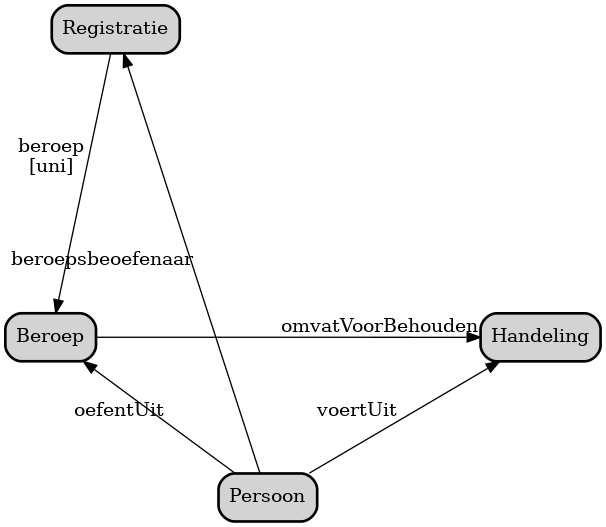
\includegraphics[scale=0.4]{04_images/CDConceptBeroep.png}
\centering
\caption{relations}
\label{fig:relations}
\end{figure}
The multiplicity must also be determined for each relation.
\begin{table}[h!]
    \begin{tabular}{||l | l||} 
     \hline
    function & The corresponding control question for the above relation $voerUit$ is\\
    \hline\hline
        Univalent & For each $Persoon$ there is at most 1 $Handeling$\\ %elke P max 1 H
        Total & For each $Persoon$ there is at least 1 $Handeling$ \\ %elke P minimaal 1 H
        Injective & For each $Handeling$ there is only 1 $Persoon$\\ %elke H max 1 P 
        Surjection & For each $Handeling$ there is at least 1 $Persoon$\\ %elke H minimaal 1 P
    \end{tabular}
    \caption{multiplicity}
    \label{tab:multiplicity}
\end{table}

By modelling using the Ampersand method, the question can be answered whether Ampersand provides more insight into the relationships.
As part of the research question, Ampersand can help you gain insight into the relationships.
Although you have to recognize and define these yourself, Ampersand will be helpful in generating functional design and prototype.
The generated prototype will validate the named constraints.
This will prevent registrations that do not meet the constraints.
These constraints are laid down in rules within Ampersand.
For example, a rule can be drawn up that determines whether a person is allowed to perform a certain action.
In figure \ref{fig:relations} the relations are named.
It was previously established that there are 2-tuple relationships.
Here we use the following notation:"$\mathit{relation [Concept \times Concept]}$".
\begin{center}
$\mathit{voertUit [Persoon \times Handeling]}$ ; 
 $\mathit{omvatVoorBehouden [Beroep \times Handeling]~\smallsmile}$
\newline $\subseteq$
\newline $\mathit{beroepsbeoefenaar [persoon \times registratie]}$ ;
$\mathit{beroep [registratie \times beroep]}$
\end{center}
The compared sets are
\newline $\mathit{[Persoon \times Beroep]}$
\newline The rule then will determine if the previous equation is true.
\newline If this is the case, then the rule is validated, otherwise the violation message occurs.
\begin{lstlisting}
    RULE HandelingDoorPersoon: voertUit; omvatVoorBehouden[Beroep*Handeling]~ |- beroepsbeoefenaar; beroep
    MEANING "Een persoon mag handelingen uitvoeren wanneer hij een bepaald beroep uitoefend"
    MESSAGE "Geen toegestane handeling."
    VIOLATION (TXT "Persoon ", SRC I, TXT " voert de handeling uit ", TGT I, TXT " die niet tot zijn beroep behoren ", SRC I[Persoon];oefentUit)
\end{lstlisting}


\subsection{Reactive approach} \label{reactive_approach}

The start of the reactive approach started with the reactive manifesto~\citepNonPub{reactive_manifesto}.
This defines the aspects that a reactive system should meet.
This includes Responsive, Resilient, Elastic and Message Driven.
These are systems that are flexible, loosely coupled and scalable and that makes them easier to develop and maintain.
Reactive Systems are made highly responsive and provide interactive feedback.
\begin{figure}[H] 
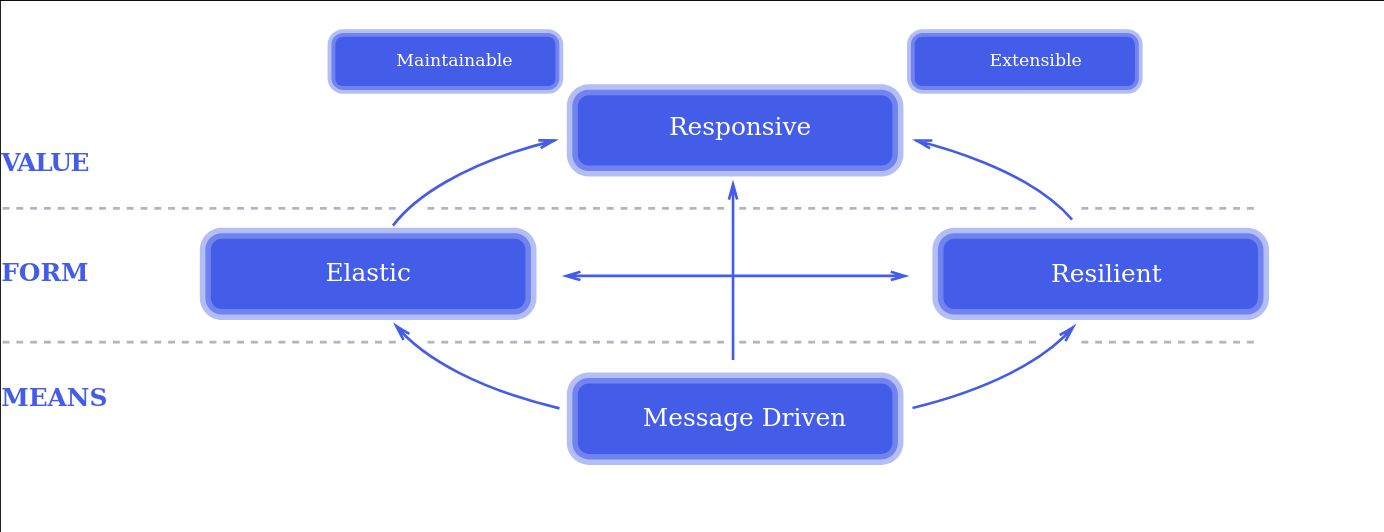
\includegraphics[scale=0.3]{04_images/reactive_manifesto.png}
\centering
\caption{reactive manifesto}
\label{fig:reactive manifesto}
\end{figure}


Ampersand is a form of Functional Reactive Programming (FRP)~\citep{elliott_functional_1997}.
The basic of reactive programming is the fact that it involves asynchronous communication.
This means that, as the \citeNonPub{reactive_manifesto} prescribes, use is made of message driven systems, but Ampersand is more than a message-driven system.
It is actually an event-driven system.
The glossary of the \citeNonPub{reactive_manifesto} indicates the difference between message driven systems and event driven systems.
An event-driven system targets event-bus while a message-driven system targets recipients~\citep{bainomugisha_survey_2013}.
The essence is that the order of the flow cannot be determined in advance.
The system will respond to events caused by constraints, Ampersand determines a dynamic flow~\citep{joosten_relation_2018}.




\subsubsection{Law analysis} \label{law_analysis}
The tax authorities have developed a method that is intended to analyse tax laws and other laws.
This is performed in these 6 steps:
\begin{enumerate}
    \item Determining the work area.
    \item Making the structure visible in legislation.
    \item Defining the meaning of legislation.
    \item Validate the analysis results.
    \item Identify missing execution policy.
    \item Setting up the knowledge model.
\end{enumerate}
Emphasis is placed on the cooperation between the implementer, ICT and policy.
By going through the method step by step, one arrives at a shared language.
This shared language includes the definition of concepts by the collaborating parties.
An important part of the approach is dividing the law into small pieces and always refer to these pieces of law in the implementation.
As a result, the method meets the requirement of the justification of government decisions.
The decisions are traceable, explainable, and it is possible to account for them.
What is not clear from the webinar~\citeNonPub{belastingdienst_webinar_2021} is how these steps were converted into an implementation.
The book~\citeNonPub{ausems_wetsanalyse_2021} indicates that the legal analysis method does not contain a development tool, but that the Tax and Customs Administration has developed an instrument based on the legal model, which is not freely available.